%% ==============================
\chapter{\iflanguage{ngerman}{Stand der Wissenschenschaft und Technik}{State of the art}}
\label{sec:state_of_the_art}
%% ==============================




Im Paper von Hong \cite{hong2003method} wird ein Approximationsbasiertes Verfahren zur Berechnung von Gradienten eines Volumens vorgestellt. 
\newline
Hierbei ist zu beachten, dass der Gradient nicht für einen Voxel direkt berechnet werden kann. Der Gradient liegt im Falle eines dreidimensionalen Volumens im Zentrum eins Würfels, der von 4 benachbarten Voxeln aufgepsannt wird. In Hongs Verfahren wird zur Berechnung die lokale 4x4x4 Nachbarschaft hinzugezogen.
\newline
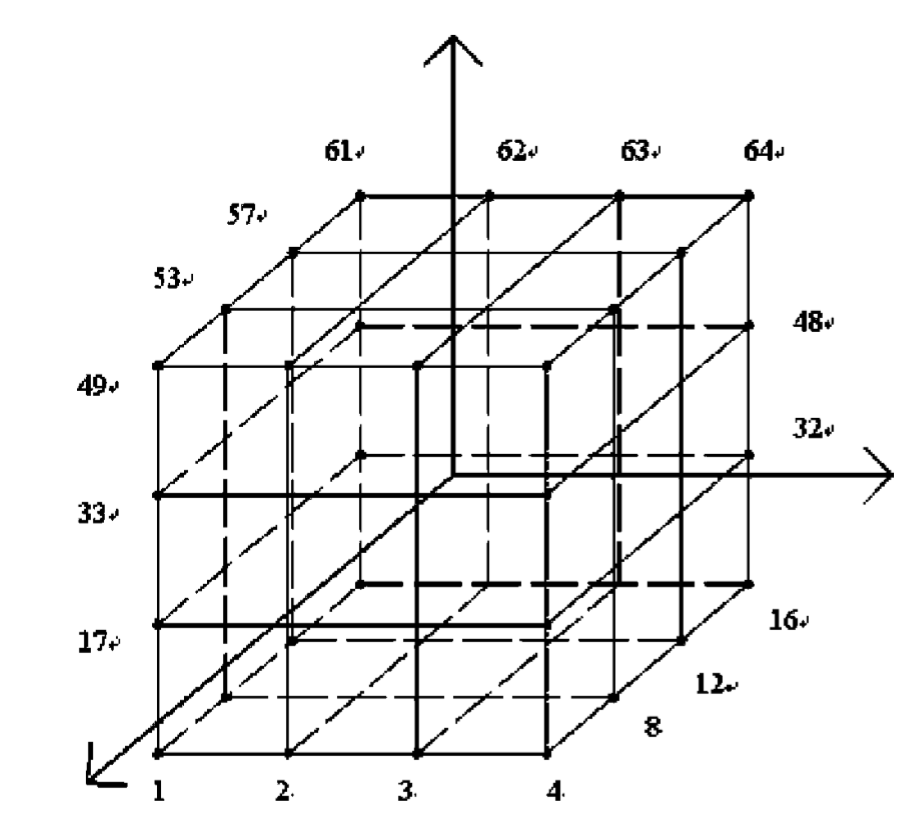
\includegraphics[width=\textwidth]{Logos/VoxelEdges.PNG}
\todo{richtig bild zitieren u. evtl kleiner}

Die Funktionen für die Intensitätswerte wird im Paper mit:  $f(x,y,z) = Ax^{2}+By^{2}+Cz^{2}+2Fyz+2Gzx+2Hxy+2Ix+2Jy+2Kz+D$  approximiert. Den dreidimensionalen Gradientenvektor n erhält man, indem man die Funktion ableitet: $n = (Ax+Gz+Hy+I, By+Fz+Hx+J, Cz + Fy + Gx + K)$ .
\newline
Um den Gradienten zu Berechnen müssen die Parameter A,B,C,E,F,G,H,I,J,K  berechnet werden. Dies geschieht mithilfe der Methode der kleinsten Quadrate.




Kindlmann und Durkin  \cite{kindlmann1998semi} - gradient


Bajaj Countour: \cite{bajaj1997contour} -1d


Correa und Ma Transferfunktion,basierend auf Größe \cite{correa2008size}, occlusion \cite{correa2009occlusion}, visibility \cite{correa2009visibility}(später histogram\cite{correa2011visibility})


Größe: 

\todo{region growing}



Imagebased:

 
Wu and Qu
proposed a system that uses editing operations and stochastic
search of the transfer function parameters to maximize the
similarity between volume-rendered images given by the user

Wu und Qu schlugen in ihrer Arbeit vor \cite{wu2007interactive}


Das Gebiet der Transferfunktionen ist weit erforscht und es existieren bereits viele verschiedene Methoden und Herangehensweisen. In diesem Abschnitt wird ein Überblick über die unterschiedlichen Vorgehensweisen von Transferfunktionen gegeben. Dabei werden diese im Folgenden in die Kategorien: eindimensionale Transferfunktionen, zweidimensionale Transferfunktionen, mehrdimensionale Transferfunktionen, ... unterteilt. Hierbei ist jedoch zu beachten, das manche der hier vorgestellten Verfahren mehrere Kategorien verbinden.


\subsection{Eindimensionale Transferfunktionen}

Die einfachste Form der Transferfunktionrm, sind die eindimensionalen Transferfunktionen. In diesen, wird nur der Intensitätswert der Voxel in Betracht gezogen. Abgesehe von den niedrigen Berechnungszeiten, sind diese jedoch aus mehreren Gründen suboptimal. Medizinischen Daten werden gemessen und haben deshalb meist ein Rauschen, was die genaue Darstellung erschwert. Weiterhin sind die Intensitätswerte verschiedener Bereiche nah beieinander oder gar gleich und damit sind eindimensionale Transferfunktionen unpraktisch um verschiedene Materialien kenntlich zu machen. Trotzdem sind eindimensionale Transferfunktionen weit verbreitet und werden oft benutzt. 

\subsection{Zweidimensionale Transferfunktionen}

Eine zweidimensionale Transferfunktion hat als Eingabeparameter zwei Werte. Oftmals werden hierbei der Gradient beziehungsweise desen Länge und der Intensitätswert eine Voxels genommen.

In der Arbeit von Wesarg und Kirschner \cite{wesarg2009structure} \cite{wesarg20102d} wird das Stucture-Size-Enhanced Histogram vorgestellt. geht es um die Benutzung von 2D Histogrammen für Transferfunktionen zur Unterscheidung von verschiedenen Gewebearten, die bei CT-Bildern ähnliche Grauwerte haben.
Dabei wird für Voxel berechnet wie viele Schritt in die jeweilige Richtung der 26 Nachbarn gemacht werden kann, ohne, dass der Grauwert um mehr als eine gewisse Differenz verändert. Die Akkumulation aller Werte ergibt dann die Größe der Struktur. Hierbei wird zur weiteren Verbesserung nur der größere Wert zweier entgegengesetzter Richtungen genommen.
Das Histogramm hat folglich als zwei Eingaben die Strukturgröße und den Grauwert.




\subsection{Mehrdimensionale Transferfunktionen}




Sereda baut seine Arbeit \cite{sereda2006visualization} auf den von Serlie \cite{serlie2003computed} vorgestellten LH-Histogramen auf und zeigt wie man mit ihnen Objekte klassifizieren kann. Die Berechnung eines LH-Histograms ist eine Methode zur Erkennung von Kanten, unter der Verwendung von Low- und High-Werten. Dabei werden die Voxel in zwei verschiedenen Kategorien eingeteilt. Es gibt Voxel, die  innerhalb eines Materials liegen und welche, die  an der Grenze zweier Materialien liegen. Ist ein Voxel innerhalb, so sind seine LH-Werte gleich. Grenzvoxel hingegen haben unterschiedliche Low- und High-Werte, wobei disese die Intensitätswerte der beiden Materialien, zwischen denen die Grenze verläuft, beschreiben. 
\newline
Bei der Berechnung des Histograms wird als erstes getestet, ob der betrachtete Voxel an einer Grenze liegt. Ein Punkt liegt innerhalb eines Materials, wenn  die Länge des Gradienten kleiner als ein gewisses epsilon (bei MRT-Daten) oder gleich null(bei CT-Daten ist). In diesem Fall wären die Low- und High-Werte der Intensitätswert des Voxels. Ist dies jedoch nicht der Fall, wird in Richtung(für die High-Werte) und entgegengesetzter Richtung(für die Low-Werte) des Gradientens schrittweise integriert. Dies stoppt sobald ein Material gefunden wurde. Dies wird für jeden Punkt im Volumen berechnet und danach aus allen LH-Werten ein Histogram erstellt.
\newline 
Zur Visualisierung benutzt Sereda eine dreidimensionale Transferfunktion. Diese nimmt die beiden LH-Werte als auch die Gradientenlänge, aus dem Grund, dass vor allem Voxel nah an der Grenze interessant sind und diese dadurch hervorgehoben werden, als Parameter entgegen.
\newline
Weiterhin verwenden die Forscher Regiongrowing um Strukturen zu erkennen. Dabei basiert die Kostenfunktion auf dem LH-Histogram. Dies ist deutlich besser als Kostenfunktionen, die auf dem Intensitätswert und der Gradientenlänge basieren, da Kanten trotz Überlappungen besser erkannt werden können.
\todo{besser schreiben}
\newline
\newline
In einer späteren Arbeit \cite{sereda2006automating} stellt Sereda ein hierarschies Clusteringverfahren vor. Hierbei werden in einer Menge von Clustern immer die zwei gemerged, die sich bei dem ausgewählten Vergleichsverfahren am ähnlichsten sind. Es wird eine Kombination aus zwei solcher Vergleichsverfahren vorgestellt. Zum einen wird die räumliche Nähe in betracht gezogen, bei der gezählt wird, wie viele direkte Nachbarn zwei Cluster besitzen. Zum anderen wird die Nähe im LH-Raum untersucht. Als Startcluster dienen hierbei die Kästchen des LH-Histograms. Die einzelnen Cluster bekommen für die Visualisierung am Ende eine zufälligen Farbwert zugewiesen. 



Die Arbeit von Shouren Lan \cite{lan2017improving} befasst sich mit der Verbesserung von 2D Transferfunktionen die auf Skalarwerten und Gradienten(SG-TF) basieren. Genauer geht es darum das Problem vom Auftauchen von Überlappungen von Bereichen die nicht zusammen gehören zu vermeiden.
\newline
Dabei wird im Paper zwischen 3 verschiedenen Arten von Strukturen unterschieden:
\begin{itemize}
\item (i) Strukturen die keine andere Struktur berühren
\item (ii) Strukturen die keine andere Struktur berühren, jedoch nah an einer andern liegen
\item (iii) Strukturen die andere Strukturen berühren
\end{itemize} 
Wenn der Benutzer eine Region ausgewählt hat, werden zunächst alle Strukturen in dem Bereich klassifiziert und kleine Fragmente entfernt. Durch verschiedene Algorithmen werden Strukturen der Klassen (ii) durch Erosion, Dilatation, Aufteilen und neu zusammenfügen von einander getrennt. Strukturen der Klasse (iii) werden durch eine weitere niedrig dimensionale Transferfunktion getrennt. Anschließend werden durch das Aufteilen entstehende Löcher mit Hilfe von Dilatation gestopft. Als letztes wird durch eine Transferfunktion den Strukturen entsprechende Farben und Intensitäten zugewiesen.


\subsection{Räumliche Info}
\subsection{Machine learning}
\subsection{Clustering basierte Transferfunktionen}


Das Paper von Binh P. Nguyen \cite{nguyen2012clustering} befasst sich mit dem Anwenden von Clustering auf einem Volumenmodell um mit Hilfe einer Transferfunktion medizinische Bilder effektiv und effizient darzustellen.
In einem Vorverarbeitungsschritt wird für jeden Voxel der Gradient berechnet, und hinterher daraus die Lower und Higher Intensitätswerte. Anschließend wird aus diesen Daten ein LH Histogramm erstellt.
In den ersten beiden Clusteringschritten werden zunächst Voxel mit ähnlichen  LH-Werten in Clustern zusammengefasst. Anschließend werden diese Cluster erneut in mehrere Cluster aufgeteilt, bei denen die Voxel auch im Raum nah beieinander liegen. Für diese beiden Schritte wird jeweils ein Parameter benötigt, der die maximale Distanz zum mittleren Voxel in einem Cluster bestimmt. Daraufhin werden alle Cluster hierarchisch gemerged, bis es nur noch einen gibt. Dabei werden immer die zwei paarweise räumlich am nächsten ausgesucht und es wird gespeichert welche Cluster gemerged wurden. Anschließend kann der Benutzer durch umkehren des Algorithmus entscheiden wie viel Cluster er haben möchte. Am Ende werden die Cluster mit verschieden Farben und Intensitätswerten versehen.

\subsection{Imagebased}
Eine weitere Art Transferfunktionen anzuwenden, sind Verfahren, die auf ?einem Bild? basieren. Hier hat der Benutzer die Möglichkeit, mit dem Programm zu interagieren. Dies ist für einen unerfahrenen User intuitiver und er kann durch ausprobieren ein gewünschtes Ergebnis erzielen.

Fang stellt in seinem Paper \cite{fang1998image} ein Verfahren vor, bei dem die  Transferfunktioneine eine Abfolge von verschieden 3D Bildverabteitungsverfahren ist, deren Parameter vom Benutzer angepasst werden können.

Es gibt auch Methoden, bei denen ein Hilfswerkzeug zum Einsatz kommt. Zum Beispiel kann der Benutzer im Paper von Reitinger: \cite{reitinger2004user} sich gezielt Bereiche des Volumens hervorheben lassen, indem er sie mit einem Stift auswählt. Hierbei wird die Intensiät des ausgewählten Punktes als auch der räumliche Abstand zum Stift in Betracht gezogen.


